\documentclass[tikz,border=2pt]{standalone}
\usepackage{newtxtext}
\usetikzlibrary{arrows.meta,positioning,fit,calc}

\definecolor{clientblue}{HTML}{DCEAF7}
\definecolor{trustgold}{HTML}{F8E7B0}
\definecolor{servergreen}{HTML}{DCEEDB}
\definecolor{riskred}{HTML}{F4D6D2}
\definecolor{ink}{HTML}{263238}

\tikzset{
  every node/.style={font=\sffamily\fontsize{7.4}{8.5}\selectfont,align=center,text=ink},
  box/.style={draw=ink!65,rounded corners=2pt,minimum height=8mm,inner sep=3pt,line width=.45pt},
  data/.style={box,fill=clientblue,minimum width=25mm},
  trust/.style={box,fill=trustgold,minimum width=31mm},
  server/.style={box,fill=servergreen,minimum width=29mm},
  outcome/.style={box,fill=riskred,minimum width=28mm},
  flow/.style={-{Stealth[length=2.2mm]},line width=.65pt,draw=ink!80},
  evidence/.style={-{Stealth[length=2.2mm]},line width=.65pt,draw=ink!80,dashed},
  group/.style={draw=ink!35,rounded corners=3pt,inner sep=4pt,line width=.5pt},
  label/.style={font=\sffamily\bfseries\fontsize{8}{9}\selectfont,anchor=west}
}

\begin{document}
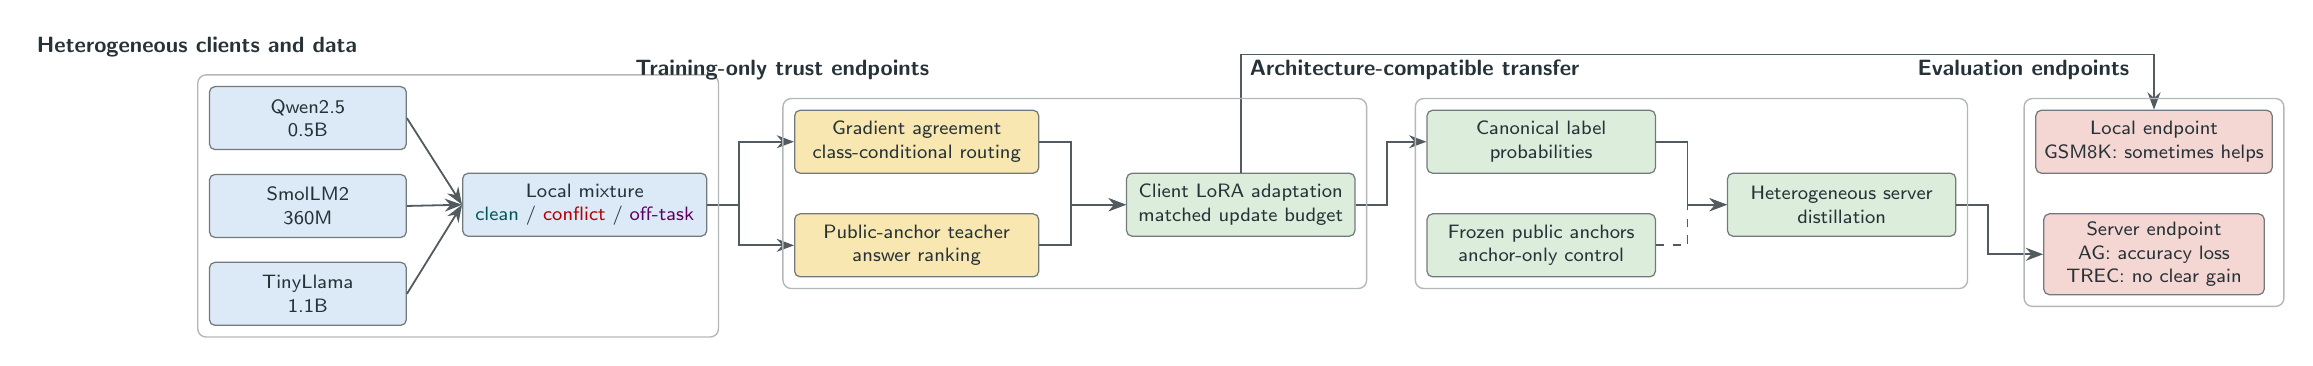
\begin{tikzpicture}[node distance=5mm and 8mm]
  \node[data] (qwen) {Qwen2.5\\0.5B};
  \node[data,below=3mm of qwen] (smol) {SmolLM2\\360M};
  \node[data,below=3mm of smol] (tiny) {TinyLlama\\1.1B};
  \node[data,right=7mm of qwen,yshift=-11mm,minimum width=31mm] (mixture)
       {Local mixture\\\textcolor{teal!70!black}{clean} / \textcolor{red!70!black}{conflict} / \textcolor{violet!75!black}{off-task}};
  \draw[flow] (qwen.east) -- (mixture.west);
  \draw[flow] (smol.east) -- (mixture.west);
  \draw[flow] (tiny.east) -- (mixture.west);

  \node[trust,right=11mm of mixture,yshift=8mm] (router)
       {Gradient agreement\\class-conditional routing};
  \node[trust,below=5mm of router] (teacher)
       {Public-anchor teacher\\answer ranking};
  \draw[flow] (mixture.east) -- ++(4mm,0) |- (router.west);
  \draw[flow] (mixture.east) -- ++(4mm,0) |- (teacher.west);

  \node[server,right=11mm of router,yshift=-8mm] (adapter)
       {Client LoRA adaptation\\matched update budget};
  \draw[flow] (router.east) -- ++(4mm,0) |- (adapter.west);
  \draw[flow] (teacher.east) -- ++(4mm,0) |- (adapter.west);

  \node[server,right=9mm of adapter,yshift=8mm] (prob)
       {Canonical label\\probabilities};
  \node[server,below=5mm of prob] (anchors)
       {Frozen public anchors\\anchor-only control};
  \draw[flow] (adapter.east) -- ++(4mm,0) |- (prob.west);

  \node[server,right=9mm of prob,yshift=-8mm] (server)
       {Heterogeneous server\\distillation};
  \draw[flow] (prob.east) -- ++(4mm,0) |- (server.west);
  \draw[evidence] (anchors.east) -- ++(4mm,0) |- (server.west);

  \node[outcome,right=10mm of server,yshift=8mm] (localout)
       {Local endpoint\\GSM8K: sometimes helps};
  \node[outcome,below=5mm of localout] (serverout)
       {Server endpoint\\AG: accuracy loss\\TREC: no clear gain};
  \draw[flow] (adapter.north) -- ++(0,15mm) -| (localout.north);
  \draw[flow] (server.east) -- ++(4mm,0) |- (serverout.west);

  \node[group,fit=(qwen)(tiny)(mixture)] (clients) {};
  \node[label,above=1mm of clients.north west] {Heterogeneous clients and data};
  \node[group,fit=(router)(teacher)(adapter)] (trustgroup) {};
  \node[label,above=1mm of trustgroup.north west] {Training-only trust endpoints};
  \node[group,fit=(prob)(anchors)(server)] (transfergroup) {};
  \node[label,above=1mm of transfergroup.north west] {Architecture-compatible transfer};
  \node[group,fit=(localout)(serverout)] (findings) {};
  \node[label,above=1mm of findings.north west] {Evaluation endpoints};
\end{tikzpicture}
\end{document}
